\documentclass[conference]{IEEEtran}
\IEEEoverridecommandlockouts
% The preceding line is only needed to identify funding in the first footnote. If that is unneeded, please comment it out.
\usepackage{acronym}

\usepackage{esvect}

\acrodef{PSO}[PSO]{\emph{particle swarm optimisation algorithm}}
\acrodef{NN}[NN]{\emph{neural network}}
\acrodef{CPSO}[CPSO]{\emph{chaotic particle swarm optimisation algorithm}}
\acrodef{RNG}[RNG]{\emph{random number generator}}
\acrodef{CPRNG}[CPRNG]{\emph{chaotic pseudo-random number generator}}
\acrodef{VN}[VN]{\emph{Von Neumann}}
\acrodef{MSE}[MSE]{\emph{mean squared error}}
\usepackage{cite}
\usepackage{amsmath,amssymb,amsfonts}
\usepackage{commath}
\usepackage{algorithmic}
\usepackage{array,multirow,graphicx}
\usepackage{textcomp}
\def\BibTeX{{\rm B\kern-.05em{\sc i\kern-.025em b}\kern-.08em
    T\kern-.1667em\lower.7ex\hbox{E}\kern-.125emX}}
\begin{document}

\title{Investigating Boundary Constraint Handling Mechanisms in Particle Swarm Optimization\\
}

\author{\IEEEauthorblockN{\\Quinton Weenink}
\IEEEauthorblockA{\textit{dept. Computer Science} \\
\textit{University of Pretoria}\\
Pretoria, South Africa \\
u13176545@tuks.co.za}
}

\maketitle

\section{Introduction}
This paper aims to investigate the effect of Boundary Constraint Handling Mechanisms on \ac{PSO}. There are many approaches that claim to improve exploration of the viable search space. In comparing these approaches to the a \ac{PSO} with no boundary constraints we could observe the changes such mechanisms are having on the performance of the \ac{PSO}.

\section{Particle Swarm Optimization}
A \ac{PSO} is a machine learning algorithm where each particle in the population represents a possible solution to the optimisation problem \cite{anna:meas-sat-nn}. Each particle moves around the search space attempting to find the optimal solution with the influence of its neighbouring particles. The position for each particle iteration is calculated as follows.

\begin{equation} \label{eq:pso:update-position}
\vec{x}_{i}^{\,t} = \vec{x}_{i}^{\,t-1} + \vec{v}_{i}^{\,t}
\end{equation}

\noindent Where:
\begin{itemize}
	\item $ \vec{x} $ is the particle position vector in n-dimensions
	\item $ \vec{v} $ is the particle velocity vector, used to calculate the particles next position
	\item $t$ is the time increment
	\item $i$ is the particle number
\end{itemize}
\vspace{5mm}
\noindent For each iteration of the algorithm, a new location of the particle is calculated based on its previous location and velocity vector as seen in (\ref{eq:pso:update-position}). The following describes a the velocity update algorithm.

\begin{equation} \label{eq:pso:update-velocity}
\vec{v}_{i}^{\,t} = w . \vec{v}_{i}^{\,t-1} + c_1 . \vec{r}_{1}^{\,t} . (\vec{x}_{pBest, i} - \vec{x}_{i}^{t-1}) + c_2 . \vec{r}_{2}^{\,t} . (\vec{x}_{nBest, i} - \vec{x}_{i}^{t-1})
\end{equation}

\noindent Where:
\begin{itemize}
	\item $c_1$ is the acceleration coefficient for the cognitive component
	\item $c_2$ is the acceleration coefficient for the social component
	\item $r_1$ and $r_2$ is a vector of random numbers in the range (0, 1)
	\item $\vec{x}_{pBest}$ is the personal best position of that particle
	\item $\vec{x}_{nBest}$ is the best position found in that particles neighbourhood
\end{itemize}
\vspace{5mm}
\noindent Particle's social component, the third term in (\ref{eq:pso:update-velocity}), requires $ nBest $, the best neighbouring particles position. The set of neighbouring particles is determined by the topology used in the \ac{PSO}. Different topologies could influence the performance of the \ac{PSO}.

Additionally, velocity max, $ V_{max} $, can be used as the limiter when calculating the particle's velocity in (\ref{eq:pso:update-velocity}), ensuring that the particle stays inside search space as well as reduce skipping over more optimal solutions. $ V_{max} $ could however prevent particles from exploring more optimal solutions.

    \subsection{Social Network Topologies}
    
    In the above mentioned \ac{PSO} the neighbourhood could be described in a variety of ways. One such method is the $ gBest $ topology, where each particle is a neighbour of every other particle in the network. This means that the particle's $ nBest $ is always the global best particle for the swarm. 
    
    Another social topology called $ lBest $ connects particles in a ring topology, the neighbourhood is specified by a fixed size of $ n_s $. The $ nBest $ in this case is determined by the best particle within $ n_s $ neighbours from the current particle\cite{vanwyk:overfitting-psoffnn}. 
    
    Finally, another social network topology exists called the \ac{VN} social network topology. This topology connects each particle to its neighbours in a lattice\cite{vanwyk:overfitting-psoffnn}. In order to determine the $ nBest $, the best error of its north, south, east and western, neighbours is used (\ref{eq:pso:update-velocity}).

	\subsection{Benchmark functions}
	
	No shifted, noisy or rotated version of the functions were used. 
	In an effort to make things scaleable different types of benchmarks functions were used in order to determine the fitness of the functions.
	
	\begin{table}[htbp]
    \caption{Benchmark functions}
    \begin{center}
    \begin{tabular}{|c|c|c|c|c|}
    \hline
    \textbf{Function}& \textbf{\textit{Multimodal}}& \textbf{\textit{Inseparable}}\\
    \hline
    Absolute value& & \\
    \hline
    Ackley& Yes& Yes\\
    \hline
    Hyperellipsoid& & \\
    \hline
    Quartic& & \\
    \hline
    Salomon& Yes& Yes\\
    \hline
    Schaffer 6& Yes& Yes\\
    \hline
    \end{tabular}
    \label{tab:nn:configuration}
    \end{center}
    \end{table}

\section{Boundary Constraint Handling Mechanisms}

The following describes the boundary constraint handling mechanisms used in this research.

\subsubsection{\textbf{No boundary constraints}}
Particles were not constrained in any way.

\subsubsection{\textbf{Feasible position update}}
Update the personal best positions only if the new particle position is better than its current personal best position, and if the new particle position is feasible. That is, a new particle position can not become
a personal best position if it violates boundary constraints.

\subsubsection{\textbf{Clamping approach}}
If a particle violates a boundary constraint in a specific dimension, then clamp the corresponding decision variable at the boundary value.

\subsubsection{\textbf{Per element reinitialization}}
For any decision variable of any particle that violates a boundary constraint, reinitialize that decision variable to a random position that satisfies the boundary constraints.

\subsubsection{\textbf{Per element reinitialization and velocity = 0}}
Adapt the per element reinitialization approach above to also set the velocity of the decision variable that violates a boundary constraint to zero. The corresponding decision variable’s new position will therefore not be influenced by the momentum term.

\subsubsection{\textbf{Initialize to personal best position}}
Initialize the boundary violating decision variable to the corresponding personal best position.

\subsubsection{\textbf{Initialize to personal best position and velocity = 0}}
Adapt the intialize to personal best position strategy above to also set the corresponding velocity to 0.

\subsubsection{\textbf{Initialize to global best position}}
Initialize to global best position: As for the above, but rather the global best for the boundary violating decision variable.

\subsubsection{\textbf{Initialize to global best position velocity = 0}}
Initialize to global best position and set velocity to zero: Adapt the intialize to global best position strategy to also set the corresponding velocity to 0.

\subsubsection{\textbf{Reverse velocity}}
The velocity of the bounadry violating decision variable is simply reversed while that decision variable violates the boundary constraint.

\subsubsection{\textbf{Arithmetic average}}
Set the bounadry violating decision variable to an arithmetic average of the corresponding personal best and global best position.

\section{Experiments}
    \subsection{\ac{PSO} configuration}
    In order to achieve viable results, each experiment was run as a mean over 50 samples. $r_1$ and $r_2$ sampled from a uniform distribution $ (0, 1) $ as specified in equation \ref{eq:pso:update-velocity}.
    
    A memory based \ac{PSO} was used with a star or $ gBest $ social topologie was used for this study. 30 particles were used for all functions. 30 dimensions were used for all functions. $ c_1 = c_2 = 1.4 $ as well $ w = 0.7 $

    No $ V_{max} $ was used

\section{Results}

\begin{table}[htbp]
\caption{Results after 5000 iterations. Means are reported over 50 samples with standard deviations in parenthesis}
\begin{center}
\begin{tabular}{|c|c|c|c|}
\hline
& $ f_1 $ & $ f_2 $ & $ f_3 $\\\hline
\multirow{2}{*}{$ BC_1 $} &
12.576554695 & 4.89108089516 & 6.6095267e-05\\
&(16.285050) & (1.948212190) & (0.00038360)\\
\hline
\multirow{2}{*}{$ BC_2 $} &
5.1857243227 & 4.58116294703 & 2.786555e-06\\
&(9.6293110) & (1.565766830) & (7.7739e-06)\\
\hline
\multirow{2}{*}{$ BC_3 $} &
57.531250757 & 6.00606880913 & 54.526024907\\
&(65.651655) & (3.434289275) & (90.3297955)\\
\hline
\multirow{2}{*}{$ BC_4 $} &
8.2467633532 & 4.55418774247 & 1.01489e-05\\
&(11.461532) & (1.648445767) & (4.589539e-05)\\
\hline
\multirow{2}{*}{$ BC_5 $} &
5.1389339174 & 4.89810256890 & 9.465576e-05\\
&(9.0355906) & (1.720959805) & (0.00032185)\\
\hline
\multirow{2}{*}{$ BC_6 $} &
9.4929921868 & 4.97768223959 & 9.924092e-06\\
&(13.040311) & (2.130050755) & (3.56359e-05)\\
\hline
\multirow{2}{*}{$ BC_7 $} &
13.266182721 & 5.07560687421 & 2.096943e-05\\
&(22.017559) & (2.252312710) & (9.81292e-05)\\
\hline
\multirow{2}{*}{$ BC_8 $} &
15.164538450 & 6.02058451060 & 0.0004165906\\
&(23.109397) & (3.086329288) & (0.00160546)\\
\hline
\multirow{2}{*}{$ BC_9 $} &
20.925653391 & 6.42808810347 & 0.0009752216\\
&(26.146772) & (3.256848326) & (0.00390649)\\
\hline
\multirow{2}{*}{$ BC_10 $} &
599.58515676 & 17.9263162102 & 797.0981965\\
&(173.65772) & (1.816182460) & (379.309663) \\
\hline
\multirow{2}{*}{$ BC_11 $} &
20.710428245 & 5.73874408816 & 15.008693567\\
&(37.284614) & (3.127739837) & (28.25022732)\\
\hline
& $ f_4 $ & $ f_4 $ & $ f_6 $\\\hline
\multirow{2}{*}{$ BC_1 $} &
1.9239946e-21 & -0.259725655 & 9.913329509\\
&(1.08892e-20) & (0.14964295) & (0.656834)\\
\hline
\multirow{2}{*}{$ BC_2 $} &
1.7858202e-26 & -0.1334162 & 9.194013340\\
&(1.1080e-25) & (0.4525834) & (0.916300)\\
\hline
\multirow{2}{*}{$ BC_3 $} &
0.37580965 & 0.2911377709212 & 10.4460088\\
&(1.8605501) & (1.837814591) & (0.7901153)\\
\hline
\multirow{2}{*}{$ BC_4 $} &
1.699433e-25 & -0.136358848 & 7.8171530590\\
&(8.329e-25) & (0.32299095) & (0.97061129)\\
\hline
\multirow{2}{*}{$ BC_5 $} &
6.203499e-20 & -0.134392611 & 9.17659654534\\
&(4.2647e-19) & (0.4148771) & (1.1028635337)\\
\hline
\multirow{2}{*}{$ BC_6 $} &
8.175363e-21 & -0.210002336 & 8.74905186834\\
&(5.722e-20) & (0.28267089) & (0.9779485313)\\
\hline
\multirow{2}{*}{$ BC_7 $} &
2.418665e-16 & -0.0636568206 & 9.9507224427\\
&(1.324e-15) & (0.466326789) & (0.798154431)\\
\hline
\multirow{2}{*}{$ BC_8 $} &
7.26727e-16 & -0.2007856567 & 10.1430737966\\
&(5.086e-15) & (0.287498829) & (0.852829383)\\
\hline
\multirow{2}{*}{$ BC_9 $} &
1.907742e-18 & -0.053840835 & 9.899939307\\
&(1.335e-17) & (0.552251796) & (0.88794107)\\
\hline
\multirow{2}{*}{$ BC_10 $} &
26.79745200 & 15.5318252566 & 12.16846579\\
&(15.81222) & (2.559650039) & (0.50818004)\\
\hline
\multirow{2}{*}{$ BC_11 $} &
4.786350e-16 & -0.2006067722 & 10.158431877\\
&(3.2479e-15) & (0.288737979) & (0.69947078)\\
\hline
\end{tabular}
\label{tab:glass}
\end{center}
\end{table}

\begin{figure}[htbp]
\centerline{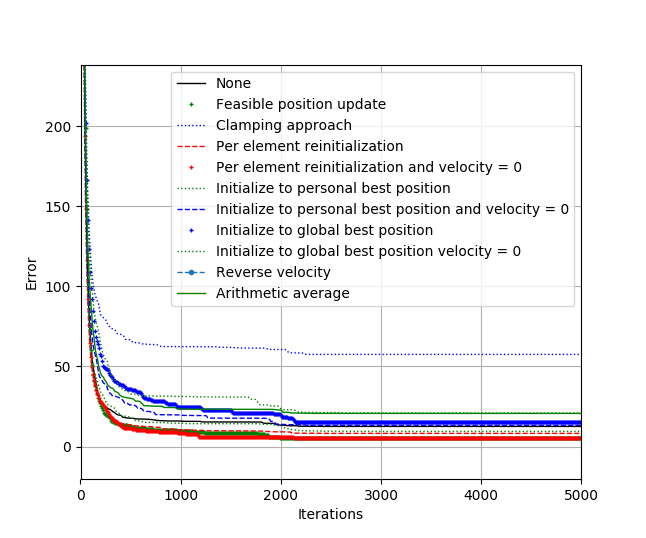
\includegraphics[width=90mm]{images/results/AbsoluteValue.png}}
\caption{$f_1$ performance}
\label{fig:absoluteValue}
\end{figure}

\begin{figure}[htbp]
\centerline{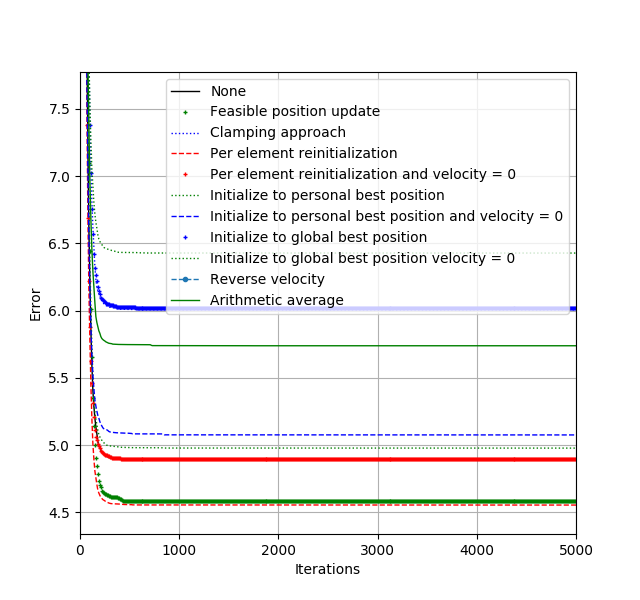
\includegraphics[width=90mm]{images/results/Ackley.png}}
\caption{$f_2$ performance}
\label{fig:ackley}
\end{figure}

\begin{figure}[htbp]
\centerline{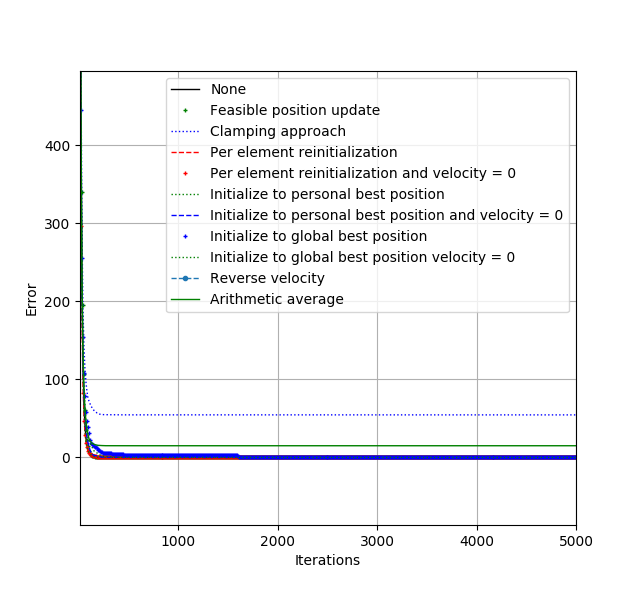
\includegraphics[width=90mm]{images/results/Hyperellipsoid.png}}
\caption{$f_3$ performance}
\label{fig:hyperellipsoid}
\end{figure}

\begin{figure}[htbp]
\centerline{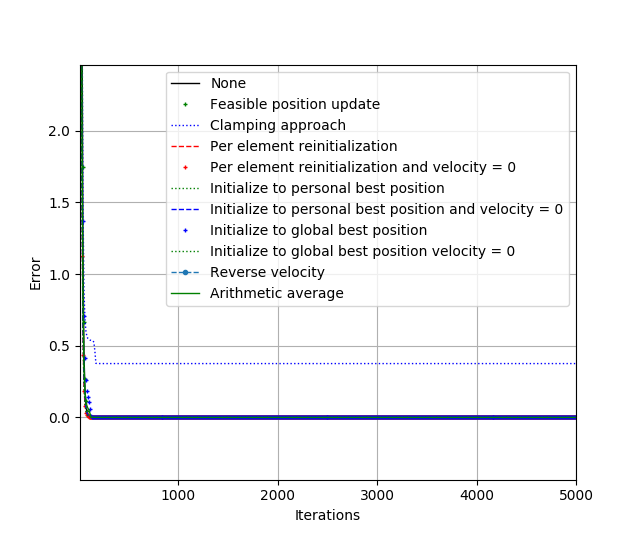
\includegraphics[width=90mm]{images/results/Quartic.png}}
\caption{$f_4$ performance}
\label{fig:quartic}
\end{figure}

\begin{figure}[htbp]
\centerline{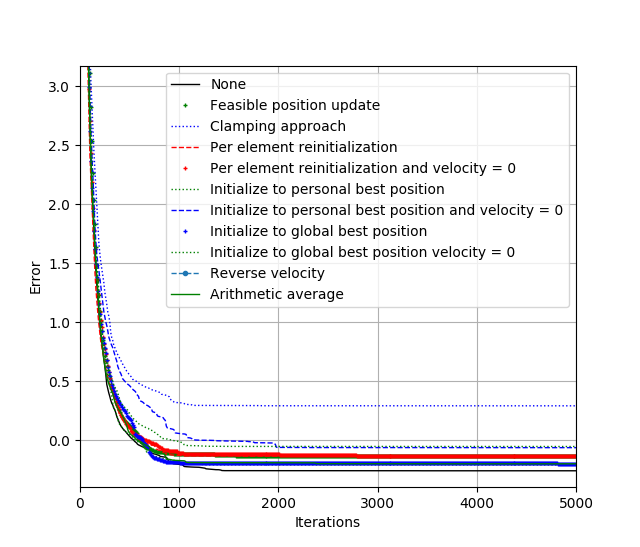
\includegraphics[width=90mm]{images/results/Salomon.png}}
\caption{$f_5$ performance}
\label{fig:salomon}
\end{figure}

\begin{figure}[htbp]
\centerline{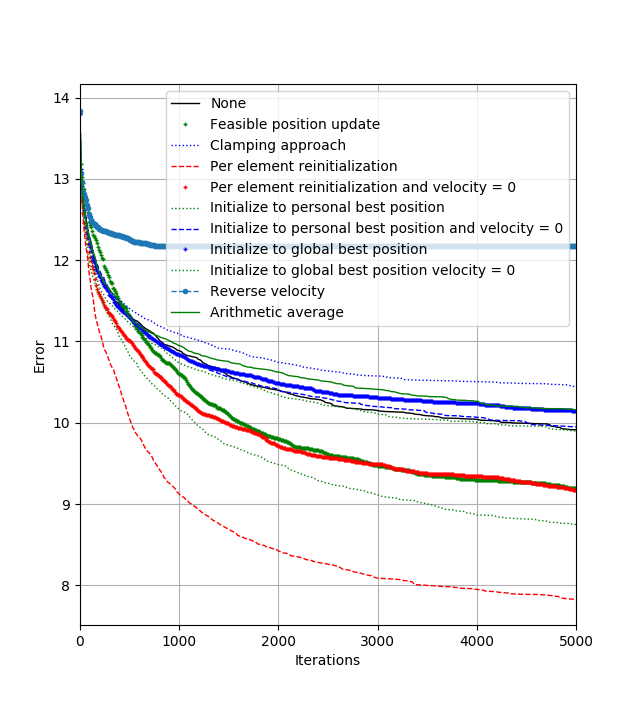
\includegraphics[width=90mm]{images/results/SchafferF6.png}}
\caption{$f_6$ performance}
\label{fig:schafferf6}
\end{figure}

\newpage
\section{Conclusion}
In conclusion one can observe that that reversing the velocity performs quite poorly and almost immediately stops exploring. Clamping which one could have been assumed to be a viable approach seemed to perform poorly on all benchmark functions.
Per-element initialisation to with out changing the velocity to zero introduces good results over all presumably due to the velocity allow it to still move towards its last found position. 

\newpage

\nocite{*}
\noindent
\bibliographystyle{IEEEtran}
\indent
\bibliography{IEEEabrv,sbc-template}

\section{Appendix}

$f_1$, the absolute value function, with $x_j \in [-100, 100]$
\begin{equation} \label{eq:function:absolute}
    f(\mathbf{x}) = \sum_{j=1}^{n_x}{\abs{x_i}}
\end{equation} 


$f_2$, the ackley function, with $x_j \in [-32.768, 32.768]$
\begin{equation} \label{eq:function:ackley}
    f(\mathbf{x}) = -20e^{-0.2\sqrt{\frac{1}{n}\sum_{j=1}^{n_x}{x_j^2}}}-e^{\frac{1}{n}\sum_{j=1}^{n_x}{cos(2\pi x_j)}} + 20 + e
\end{equation}

$f_n$, the hyperellipsoid function, with $x_j \in [−5.12, 5.12]$
\begin{equation} \label{eq:function:hyperellipsoid}
    f(\mathbf{x}) = \sum_{j=1}^{n_x}{jx_j^2}
\end{equation}

$f_n$, the quartic function, with $x_j \in [−5.12, 5.12]$
\begin{equation} \label{eq:function:hyperellipsoid}
    f(\mathbf{x}) = \sum_{j=1}^{n_x}{jx_j^4}
\end{equation}

$f_n$, the salomon function, with $x_j \in [-100, 100]$
\begin{equation} \label{eq:function:salomon}
    f(\mathbf x)=-cos(2\pi\sum_{j=1}^{n_x}x_j^2)+0.1\sqrt{\sum_{j=1}^{n_x}x_j^2}
\end{equation}

$f_n$, the schaffer 6 function, with $x_j \in [-100, 100]$
\begin{equation} \label{eq:function:schafferf6}
    f(x,y)=\sum_{j=1}^{n_x}{\left(0.5+\frac{sin^2(\sqrt{x^2 + y^2})-0.5}{[1+0.001 \cdot (x^2 + y^2)]^2}\right)}
\end{equation}

\end{document}
